\documentclass[11pt]{article}

\usepackage[margin=0.9in]{geometry}
\usepackage{setspace}
\setstretch{1.02}
\usepackage{booktabs}
\usepackage{graphicx}
\usepackage{caption}
\usepackage{float}
\usepackage{array}
\usepackage{longtable}
\usepackage[hidelinks]{hyperref}
\hypersetup{pdftitle={Training-Free Token Reduction on MotionBench: Results},
            pdfauthor={VLLM Project}}

\captionsetup{font=small,labelfont=bf}

\title{Training-Free Token Reduction on MotionBench\\
\large Results}
\author{VLLM Project}
\date{\today}

\begin{document}
\maketitle

\noindent Eleven training-free video-LLM token-reduction methods, evaluated
on MotionBench (8{,}052 questions, 4{,}018 scoreable) across two backbones
--- LLaVA-OV-7B and Qwen3-VL-8B --- at 32 frames. Results only: full
methodology, the verification gate, and limitations are in \texttt{paper.tex}.
At $n=4{,}018$ the binomial 95\% confidence half-width is $\pm1.54$ points;
$^{*}$ marks a difference significant by McNemar's test on paired predictions
($\chi^2\geq3.84$, $p<0.05$).

\tableofcontents

% =====================================================================
\section{Common settings}
\label{sec:settings}

Held fixed across every method and both backbones:

\begin{itemize}
  \setlength\itemsep{0.15em}
  \item \textbf{32 frames}, sampled uniformly per video.
  \item \textbf{Greedy decoding} (\texttt{do\_sample=False}, \texttt{max\_new\_tokens=16}), batch size 1.
  \item \textbf{Letter-match scoring} (A--D) against ground truth; the 4{,}034 \texttt{NA} items are excluded, leaving 4{,}018 scoreable.
  \item Methods exposing a single retention knob are standardized to \textbf{15\% nominal retention}; methods with no such knob (frame-selection methods, or methods whose budget is fixed internally) keep their published defaults --- forcing 15\% on those would break paper fidelity.
\end{itemize}

Per-method settings, mechanisms and measured token budgets are in
Table~\ref{tab:permethod} (\S\ref{sec:permethod}).

% =====================================================================
\section{Master table}
\label{sec:master}

Table~\ref{tab:llava} and Table~\ref{tab:qwen}: every method at its
standardized 15\% or published default, one table per backbone; footnotes
mark exceptions (frame-selection methods, no-knob methods, published
alternate points). Full retention sweeps are in \S\ref{sec:retentionsec}.

\begin{table}[H]
  \centering
  \small
  \caption{LLaVA-OV-7B, 32 frames, 15\% nominal retention except where
  noted. AO = Action Order, CM = Camera Motion, LM = Location-related
  Motion, MR = Motion Recognition, MO = Motion-related Objects, RC =
  Repetition Count (\% correct within category, chance = 25\%). $\Delta$ is
  vs.\ baseline. $^{*}$ = significant. $^{\S}$ AIM: 25\% retention (two
  active merge steps ship in the released code). $^{\dagger}$ PruneVID-OV:
  \texttt{cluster\_ratio=0.5} (50\%), the authors' only published point.
  $^{\ddagger}$ no retention knob; one fixed recipe (Table~\ref{tab:permethod}).
  $^{\P}$ VisionZip is the contextual half only --- no CLS token to select
  the dominant half (same as the Qwen3-VL cell, Table~\ref{tab:qwen}).}
  \label{tab:llava}
  \begin{tabular}{lrrrrrrrr}
    \toprule
    Method & Overall & $\Delta$ & AO & CM & LM & MR & MO & RC \\
    \midrule
    \textit{Baseline} & \textit{52.66} & --- & \textit{40.5} & \textit{45.2} & \textit{55.5} & \textit{57.0} & \textit{71.2} & \textit{23.8} \\
    DyCoke$^{\ddagger}$ & 53.36 & +0.70 & 38.9 & 48.8 & 55.7 & 58.2 & 70.9 & 25.2 \\
    FlashVID & 53.31 & +0.65 & 39.9 & 45.7 & 53.8 & 58.0 & 71.7 & 28.2 \\
    HoliTom & 53.14 & +0.47 & 40.8 & 49.6 & 52.6 & 57.0 & 71.4 & 27.3 \\
    MDP3 & 53.06 & +0.40 & 40.5 & 49.6 & 53.5 & 56.8 & 71.6 & 26.5 \\
    VideoITG & 52.86 & +0.20 & 40.1 & 47.0 & 53.7 & 57.6 & 70.1 & 26.8 \\
    AIM$^{\S}$ & 52.86 & +0.20 & 41.4 & 48.1 & 54.2 & 57.0 & 71.9 & 22.2 \\
    VisionZip (ctx.)$^{\P}$ & 51.79 & --0.87 & 40.1 & 46.2 & 53.7 & 56.2 & 69.4 & 23.2 \\
    STTM$^{\ddagger}$ & 51.72 & --0.95 & 39.9 & 48.1 & 53.8 & 53.5 & 70.6 & 28.7 \\
    PruneVID-OV$^{*\dagger}$ & 37.53 & --15.13 & 31.2 & 34.0 & 35.7 & 38.0 & 52.0 & 24.8 \\
    FastV$^{*}$ & 36.78 & --15.88 & 32.8 & 31.9 & 34.1 & 35.7 & 53.8 & 25.2 \\
    \bottomrule
  \end{tabular}
\end{table}

\begin{table}[H]
  \centering
  \small
  \caption{Qwen3-VL-8B, 32 frames, 15\% nominal retention except where
  noted. All ten portable methods. VisionZip is the contextual half only,
  as in Table~\ref{tab:llava}. FlashVID and STTM run the authors' own code
  at published settings (\S\ref{sec:permethod}). $^{\dagger}$ PruneVID:
  \texttt{cluster\_ratio=0.5} (50\%), the authors' only published point.
  $^{\ddagger}$ no retention knob; one fixed recipe (Table~\ref{tab:permethod}).}
  \label{tab:qwen}
  \begin{tabular}{lrrrrrrrr}
    \toprule
    Method & Overall & $\Delta$ & AO & CM & LM & MR & MO & RC \\
    \midrule
    \textit{Baseline} & \textit{62.52} & --- & \textit{46.1} & \textit{63.1} & \textit{65.0} & \textit{67.3} & \textit{79.0} & \textit{33.8} \\
    PruneVID$^{\dagger}$ & 62.17 & --0.35 & 46.1 & 62.9 & 64.1 & 67.1 & 79.1 & 32.5 \\
    DyCoke$^{\ddagger}$ & 61.85 & --0.67 & 45.1 & 62.6 & 63.9 & 66.4 & 78.4 & 34.5 \\
    STTM$^{*\ddagger}$ & 61.60 & --0.92 & 45.9 & 61.6 & 64.8 & 66.0 & 77.1 & 34.8 \\
    HoliTom$^{*}$ & 60.33 & --2.19 & 44.7 & 61.3 & 61.0 & 66.4 & 76.2 & 29.0 \\
    MDP3$^{*}$ & 59.66 & --2.86 & 44.9 & 64.7 & 62.8 & 64.0 & 77.4 & 23.0 \\
    FlashVID$^{*}$ & 59.36 & --3.16 & 43.5 & 57.4 & 62.6 & 65.6 & 77.2 & 23.5 \\
    FastV$^{*}$ & 59.01 & --3.51 & 46.2 & 61.0 & 61.9 & 63.5 & 72.2 & 30.5 \\
    VisionZip (ctx.)$^{*}$ & 58.81 & --3.71 & 43.2 & 57.4 & 61.9 & 64.2 & 74.3 & 29.5 \\
    VideoITG$^{*}$ & 56.35 & --6.17 & 45.3 & 53.5 & 59.3 & 60.2 & 75.4 & 22.2 \\
    AIM$^{*}$ & 55.97 & --6.55 & 45.9 & 56.6 & 59.5 & 58.3 & 72.2 & 27.0 \\
    \bottomrule
  \end{tabular}
\end{table}

\subsection{Retention sweep}
\label{sec:retentionsec}

Three methods (FastV, FlashVID, HoliTom) have a retention knob the authors
validate at more than one point; each is run at every point they publish,
not just 15\%. Table~\ref{tab:sweepllava} and Table~\ref{tab:sweepqwen} are
that data, one table per backbone; baseline is in Table~\ref{tab:llava}/
\ref{tab:qwen} above, not repeated here.

\begin{table}[H]
  \centering
  \small
  \caption{LLaVA-OV-7B retention sweep (baseline 52.66\%). $^{*}$ =
  significant. FastV's range is its authors' full published boundary,
  re-run with the \texttt{PrunableDynamicCache} fix (\S\ref{sec:permethod})
  --- every point reproduces its pre-fix value almost exactly. FlashVID and
  HoliTom publish 10/15/20/25\% on every backbone they support; VisionZip
  (contextual-only, \S\ref{sec:master}) was swept over the same range for
  this report.}
  \label{tab:sweepllava}
  \begin{tabular}{lrrrrrr}
    \toprule
    Method & 10\% & 15\% & 20\% & 25\% & 50\% & 75\% \\
    \midrule
    FastV & 36.06$^{*}$ & 36.78$^{*}$ & 36.93$^{*}$ & 36.73$^{*}$ & 36.31$^{*}$ & 35.69$^{*}$ \\
    FlashVID & 52.51 & 53.31 & 53.71$^{*}$ & 53.36 & --- & --- \\
    HoliTom & 52.76 & 53.14 & 53.06 & 53.41 & --- & --- \\
    VisionZip (ctx.) & 51.69 & 51.79 & 51.92 & 52.54 & --- & --- \\
    \bottomrule
  \end{tabular}
\end{table}

\begin{table}[H]
  \centering
  \small
  \caption{Qwen3-VL-8B retention sweep (baseline 62.52\%). $^{*}$ =
  significant. All four FlashVID cells now use the authors'-code
  implementation (\S\ref{sec:permethod}), the same one that produced the
  15\% cell elsewhere in this report --- monotonic in retention. FlashVID
  and HoliTom are not published beyond 25\% on this backbone.}
  \label{tab:sweepqwen}
  \begin{tabular}{lrrrrrr}
    \toprule
    Method & 10\% & 15\% & 20\% & 25\% & 50\% & 75\% \\
    \midrule
    FastV & 56.92$^{*}$ & 59.01$^{*}$ & 59.83$^{*}$ & 60.60$^{*}$ & 62.32 & 62.64 \\
    FlashVID & 58.04$^{*}$ & 59.36$^{*}$ & 60.05$^{*}$ & 60.70$^{*}$ & --- & --- \\
    HoliTom & 60.05$^{*}$ & 60.33$^{*}$ & 60.38$^{*}$ & 60.43$^{*}$ & --- & --- \\
    \bottomrule
  \end{tabular}
\end{table}

FlashVID's 20\% cell is a small local peak on LLaVA-OV (53.71\% vs.\
53.31\%/53.36\% at 15\%/25\%), gate-clean but not persisting outside 20\%.
On Qwen3-VL it's instead cleanly monotonic (58.04$\to$60.70\% over
10--25\%). HoliTom shows no such bump on either backbone. VisionZip's
sweep (51.69--52.54\%) is gentle and never significant --- unlike FastV
and PruneVID-OV, it does not collapse on LLaVA-OV. FastV is the sharpest
backbone contrast here: collapsed at 50\%/75\% on LLaVA-OV
(35.7--36.3\%) but at baseline parity on Qwen3-VL (62.32\%/62.64\%, not
significant) --- the same rule that permanently breaks the model on one
backbone is harmless by half retention on the other.

PruneVID publishes one operating point (\texttt{cluster\_ratio=0.5}, its
row in Table~\ref{tab:llava}/\ref{tab:qwen}); we additionally swept it at
10\%/25\% (not authors'-validated) and found the same backbone split as
FastV: monotonic on Qwen3-VL ($60.23\to61.40\to62.17\%$), collapsed
throughout on LLaVA-OV ($37.88\to37.53\to37.53\%$, all $>14$ points below
baseline).

Tripling FastV's budget from 10\% to 25\% moves it 3.68 points on Qwen3-VL,
against no more than 0.85 points for any LLaVA-OV method over the same
range --- the two backbones respond to retention completely differently.

% =====================================================================
\section{Figures}
\label{sec:figures}

\begin{figure}[H]
  \centering
  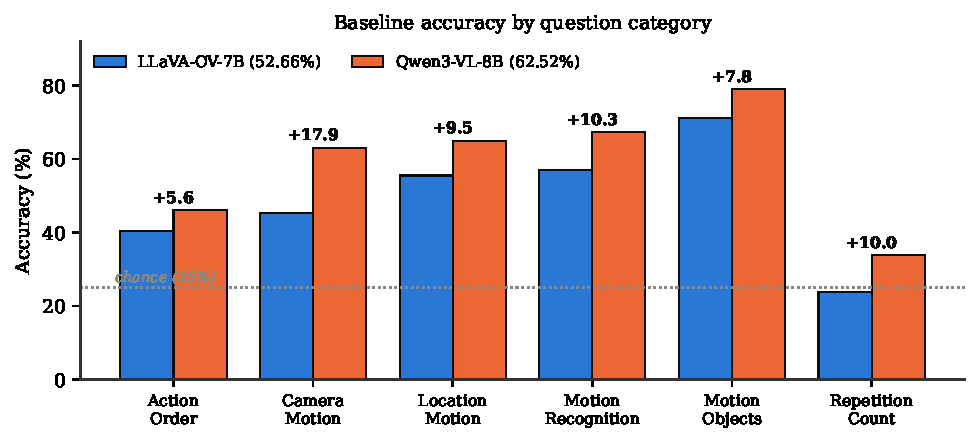
\includegraphics[width=0.86\linewidth]{figures/r3_fig1_baseline_color.pdf}
  \caption{Baseline accuracy by category, both backbones (bar).}
  \label{fig:baseline}
\end{figure}

\begin{figure}[H]
  \centering
  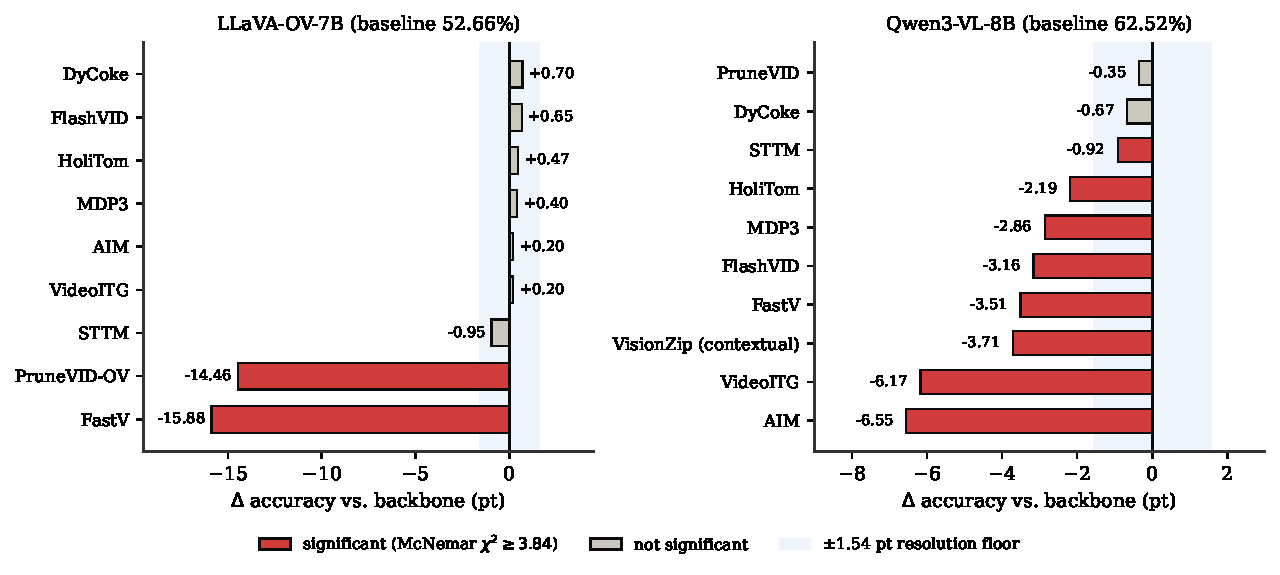
\includegraphics[width=\linewidth]{figures/r3_fig2_delta_color.pdf}
  \caption{Change vs.\ backbone, every method, both backbones (bar). Red =
  significant by McNemar's test; the shaded band is the $\pm1.54$-point
  resolution floor.}
  \label{fig:delta}
\end{figure}

\begin{figure}[H]
  \centering
  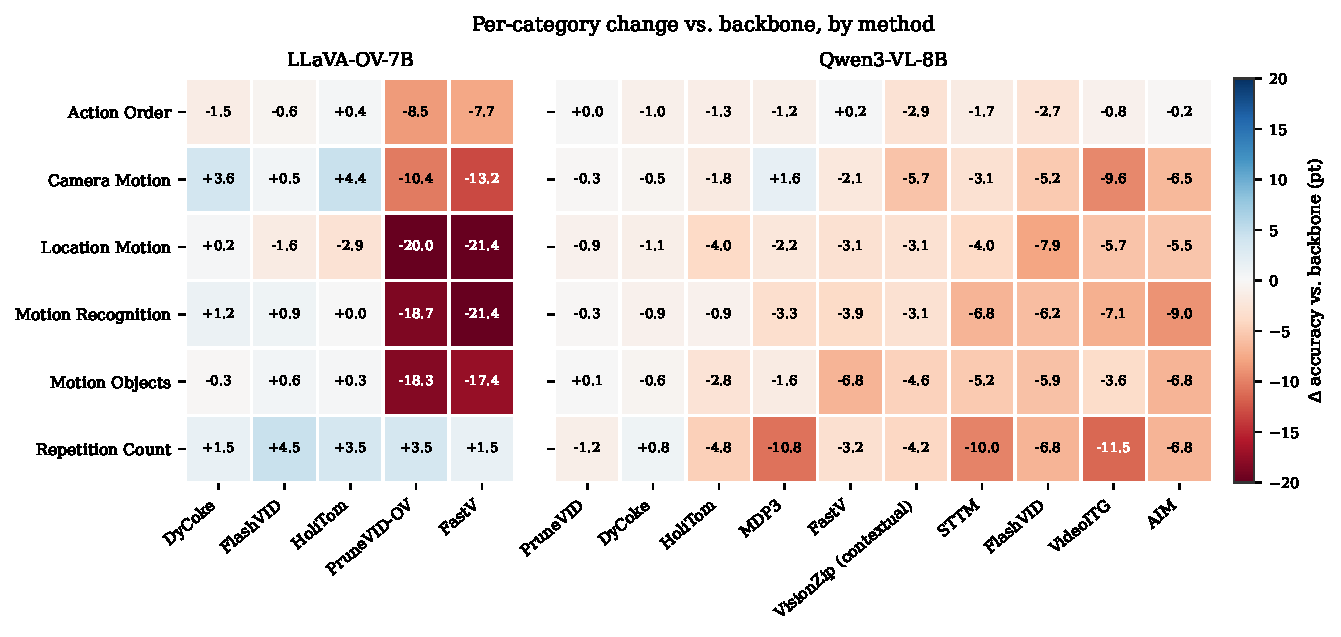
\includegraphics[width=\linewidth]{figures/fig3_category_delta.pdf}
  \caption{Per-category change vs.\ backbone, by method (heatmap). Blue =
  gain, red = loss.}
  \label{fig:heatmap}
\end{figure}

\begin{figure}[H]
  \centering
  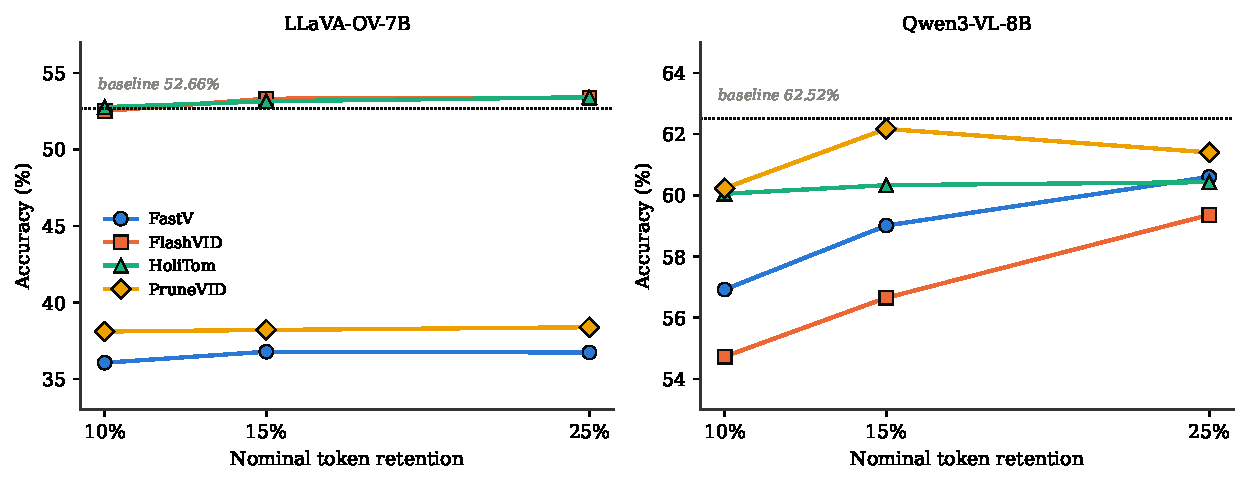
\includegraphics[width=\linewidth]{figures/r3_fig3_retention_color.pdf}
  \caption{Accuracy against nominal token retention, the four methods with a
  retention knob (dot + line).}
  \label{fig:retention}
\end{figure}

\begin{figure}[H]
  \centering
  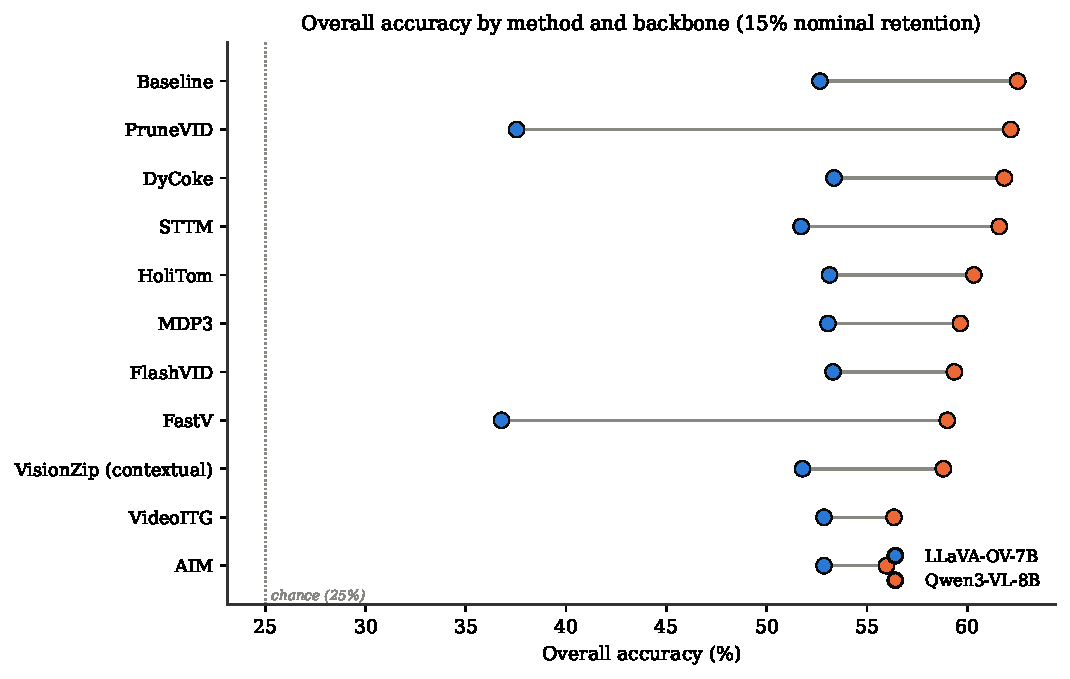
\includegraphics[width=0.86\linewidth]{figures/r3_fig4_dotplot_methods.pdf}
  \caption{Overall accuracy by method and backbone at 15\% nominal retention
  (Cleveland dot plot). Rows sorted by Qwen3-VL accuracy; the line spans each
  method's two backbone results.}
  \label{fig:dotplot}
\end{figure}

% =====================================================================
\section{Per-method settings}
\label{sec:permethod}

Table~\ref{tab:permethod} is the mechanism and exact configuration behind
every row above.

\begin{table}[H]
  \centering
  \footnotesize
  \caption{Per-method mechanism, key parameters (as run in this report), and
  measured visual-token budget. Budgets are read from each method's
  execution log on Qwen3-VL-8B (11{,}664 visual input tokens at 32 frames),
  not from its CLI flag --- nominal 15\% describes the configured knob, not
  necessarily what is actually retained. Frame-selection methods have no
  token budget to measure; they instead reduce the number of frames fed to
  the model.}
  \label{tab:permethod}
  \begin{tabular}{p{2.1cm}p{3.9cm}p{4.8cm}p{2.7cm}}
    \toprule
    Method & Mechanism & Key parameters (this report) & Measured\newline budget \\
    \midrule
    HoliTom & pre-LLM segment retain $+$ in-LLM merge & \texttt{RETAIN\_RATIO=0.15 T=0.80 HOLITOM\_k=18 HOLITOM\_r=0.5} & 7.5\% (875 tok.) \\
    STTM & quadtree spatio-temporal merge & LLaVA-OV: \texttt{thresh=0.85 temporal=0.65 root=1}. Qwen3-VL: \texttt{thresh=0.85 temporal=0.65 root=2} --- a published setting (\texttt{s3\_sttm\_pub\_run}), replacing an earlier off-spec \texttt{root=0, temporal=--1.0} cell & 9.0\% (1{,}050 tok.) on LLaVA-OV; not re-measured at the corrected Qwen3-VL setting \\
    FastV$^{\ddagger}$ & in-LLM attention rerank, layer 2 & \texttt{K=2, R=0.85} (keep 15\%). Re-run with the \texttt{PrunableDynamicCache} fix; K=2/R=50\% (36.31\%) and K=2/R=75\% (35.69\%) were also run and land in the same collapse band (Table~\ref{tab:sweepllava}) & 15.0\% (1{,}750 tok.) \\
    FlashVID & pre-LLM temporal-segment merge $+$ inner-LLM compression, layer 28 & authors' \texttt{flashvid()} package: \texttt{retention\_ratio=0.15 alpha=0.7 temporal\_threshold=0.8 token\_selection\_method=attn\_div pruning\_layer=28 llm\_retention\_ratio=0.1 expansion=1.25 min\_segment\_num=4} & 15.0\% (1{,}750 tok.) pre-LLM; the layer-28 stage compresses surviving visual tokens by a further 90\% mid-network, not captured by this single figure \\
    AIM & bipartite merge $+$ PageRank prune & 2-step merge schedule compiled in; no CLI retention knob. Qwen3-VL 15\%; LLaVA-OV 25\% (ships two active steps) & 15.0\% (1{,}750 tok.) \\
    VisionZip (contextual) & key-similarity merge in the vision tower & LLaVA-1.5-7B (native): \texttt{dominant=54 contextual=10} at 8 frames. LLaVA-OV \& Qwen3-VL: contextual-only port, \texttt{retention\_ratio=0.15} --- neither vision tower has a CLS token to select the dominant half & 15.0\% (1{,}750 tok.) \\
    DyCoke & temporal merge $+$ KV prune, layer 3 & \texttt{l=3 p=0.7 k=0.7}; no single retention knob, net $\sim$49\% & 49.0\% (5{,}716 tok.) \\
    PruneVID & DPC-KNN cluster merge, layer 10 & \texttt{cluster=0.50 seg=0.25}; LLaVA-OV port has no upstream reference (upstream targets PLLaVA only) & 50.0\% (5{,}832 tok.) \\
    \midrule
    MDP3 & frame selection (DPP) & \texttt{pool=32 select=8} --- selects frames, not tokens & n/a (8 of 32 frames) \\
    VideoITG & grounded frame selection & 512 sampled $\to$ 32 selected & n/a (32 of 512 sampled) \\
    DyTo\textsuperscript{$\dagger$} & FINCH clustering $+$ ToMe token merge & \texttt{temporal\_aggregation=}\allowbreak\texttt{spatial\_\allowbreak tome\_\allowbreak finch\_\allowbreak dynamic\_\allowbreak all\_frms}; own Vicuna-7B backbone & $\sim$3{,}680 tok.\ from 100 input frames \\
    \bottomrule
  \end{tabular}

  \bigskip
  \footnotesize $^{\dagger}$ DyTo does not run on either standardized backbone; listed here for completeness (see Table~\ref{tab:native}). $^{\ddagger}$ every prior LLaVA-OV FastV run silently discarded its own pruning (a \texttt{PrunableDynamicCache} bug, \S\ref{sec:notable}); re-run with the fix, every point reproduces its pre-fix value almost exactly.
\end{table}

% =====================================================================
\section{Correct/incorrect vs.\ baseline}
\label{sec:paired}

\emph{Fixed} = wrong under the baseline, correct under the method.
\emph{Broke} = correct under the baseline, wrong under the method. Both are
McNemar discordant pairs on the 4{,}018 scoreable items. \emph{Differ} counts
predictions unequal to the baseline's over all 8{,}052 rows (0 would mean a
silent no-op --- see \texttt{paper.tex} for the verification gate this
guards against).

\begin{table}[H]
  \centering
  \small
  \caption{Paired-prediction statistics against each backbone's baseline.}
  \label{tab:verif}
  \begin{tabular}{lrrrrl}
    \toprule
    Method & Differ & Fixed & Broke & $\chi^2$ & Significant \\
    \midrule
    \multicolumn{6}{l}{\textit{LLaVA-OV-7B}} \\
    DyCoke & 1{,}031 & 170 & 142 & 2.34 & no \\
    FlashVID & 1{,}610 & 268 & 242 & 1.23 & no \\
    HoliTom & 1{,}838 & 299 & 280 & 0.56 & no \\
    MDP3 & 1{,}452 & 246 & 230 & 0.47 & no \\
    VideoITG & 1{,}193 & 192 & 184 & 0.13 & no \\
    AIM & 1{,}406 & 227 & 219 & 0.11 & no \\
    STTM & 4{,}859 & 329 & 367 & 1.97 & no \\
    VisionZip (ctx.) & 1{,}725 & 260 & 295 & 2.08 & no \\
    PruneVID-OV & 5{,}075 & 448 & 1{,}056 & 244.98 & yes \\
    FastV & 4{,}701 & 475 & 1{,}113 & 255.52 & yes \\
    \midrule
    \multicolumn{6}{l}{\textit{Qwen3-VL-8B}} \\
    PruneVID & 1{,}074 & 56 & 70 & 1.34 & no \\
    DyCoke & 1{,}048 & 83 & 110 & 3.50 & no \\
    HoliTom & 1{,}657 & 131 & 219 & 21.63 & yes \\
    MDP3 & 1{,}626 & 159 & 274 & 30.01 & yes \\
    FastV & 2{,}029 & 149 & 290 & 44.65 & yes \\
    VisionZip (contextual) & 2{,}035 & 191 & 340 & 41.25 & yes \\
    STTM & 1{,}510 & 133 & 170 & 4.28 & yes \\
    FlashVID & 2{,}069 & 157 & 284 & 36.00 & yes \\
    VideoITG & 2{,}522 & 206 & 454 & 92.44 & yes \\
    AIM & 2{,}861 & 194 & 457 & 105.44 & yes \\
    \midrule
    \multicolumn{6}{l}{\textit{Backbone vs.\ backbone}} \\
    Qwen3-VL-8B vs.\ LLaVA-OV-7B & 7{,}081 & 810 & 414 & 127.47 & yes \\
    \bottomrule
  \end{tabular}
\end{table}

Divergence volume does not predict damage. STTM on LLaVA-OV changes 4{,}859
predictions --- more than FastV's 4{,}701 --- yet loses 0.95 points and is
not significant, because its changes fall almost evenly in both directions
(329 fixed, 367 broken). FastV changes a comparable number destructively
(475 fixed, 1{,}113 broken).

% =====================================================================
\section{Methods on non-standard backbones}
\label{sec:native}

\begin{table}[H]
  \centering
  \small
  \caption{Runs on backbones other than the two standardized ones. Not
  comparable to Tables~\ref{tab:llava}--\ref{tab:qwen}; no $\Delta$ is given
  because no matched baseline exists for any row. PruneVID's released code
  targets PLLaVA only --- this is the authors' real backbone and the one
  cell with an upstream reference to validate against, unlike the LLaVA-OV
  port (PruneVID-OV, Table~\ref{tab:llava}).}
  \label{tab:native}
  \begin{tabular}{llrrrrrrr}
    \toprule
    Method & Backbone & Overall & AO & CM & LM & MR & MO & RC \\
    \midrule
    VisionZip & LLaVA-1.5-7B & 40.09 & 33.7 & 33.0 & 37.2 & 41.1 & 57.4 & 25.8 \\
    PruneVID & PLLaVA-7B & 44.13 & 35.6 & 33.0 & 41.0 & 47.0 & 63.3 & 26.5 \\
    DyTo (recon.\ TW-FINCH) & Vicuna-7B & 42.06 & 32.4 & 33.0 & 42.1 & 43.0 & 61.7 & 26.0 \\
    \bottomrule
  \end{tabular}
\end{table}

% =====================================================================
\section{Notable}
\label{sec:notable}

The backbone swap moves accuracy 9.86 points --- more than any
token-reduction method moves it, either direction, either backbone, any
retention level tested. Rankings do not transfer: PruneVID is the worst
LLaVA-OV result (37.53\%) and the best Qwen3-VL one ($-0.35$);
Figure~\ref{fig:dotplot} shows the crossing lines directly. FastV and
PruneVID-OV collapse specifically on LLaVA-OV (36.8--37.5\%, $>15$ points
below baseline, significant), while every other LLaVA-OV method is statistically
indistinguishable from the backbone; FastV's own published range does not
save it (35.7--36.3\% at 75\% and 50\% keep, Table~\ref{tab:sweepllava}).
Qwen3-VL inverts the pattern: every method loses, eight of ten losses are
significant, but none approaches the LLaVA-OV collapse --- the largest
Qwen3-VL loss (AIM, $-6.55$) is smaller than the smallest LLaVA-OV collapse.

Only three methods qualify as having an authors'-validated retention sweep
(\S\ref{sec:retentionsec}); the other five with any
retention-like parameter do not. \textbf{PruneVID} publishes exactly one
ratio. \textbf{DyCoke} has no
single retention knob, only one fixed three-parameter recipe. \textbf{AIM}
has no knob at all on LLaVA-OV and an unpublished, self-ported one on
Qwen3-VL. \textbf{STTM} is configured per-benchmark, not a sweepable
percentage. \textbf{VisionZip}'s contextual-only port does have a
sweepable ratio, but the authors never validate one --- our 10--25\% sweep
(Table~\ref{tab:sweepllava}) is ours, not theirs.

\paragraph{A cache bug silently discarded FastV's and PruneVID's pruning on
LLaVA-OV, not that it mattered.} Both prune via a shared
\texttt{PrunableDynamicCache} class whose \texttt{update()} pruned only
what it returned to attention, not what it stored --- so the pruning was
lost every time the cache round-tripped through
\texttt{generate()}'s legacy-tuple export, and every decode step ran
fully unpruned. (PruneVID had a second bug on top: a stray
\texttt{dycoke=True} left over from a copy-pasted loader, which reset its
cache every decode step and crashed once the first bug stopped masking
it.) Both are fixed --- prune is now physical, survives the round-trip, and
the stray flag is removed. Re-running FastV's full range with the fix
reproduces every pre-fix number to within 0.03\%: the LLaVA-OV collapse is
genuine model behavior, not the bug. PruneVID needed one more fix on top:
the \texttt{lengeh\_vision\_token} kwarg both methods used to locate the
visual-token span turns out to be hard-coded \texttt{None} by
\texttt{prepare\_inputs\_labels\_for\_multimodal()} for every caller ---
FastV's own working fallback (arithmetic from a fixed text tail) had to be
ported over. With every fix applied, PruneVID's LLaVA-OV sweep lands at
37.53--37.88\%, within 0.9 points of its pre-fix numbers
(38.10--38.38\%): same conclusion, genuine collapse. Qwen3-VL is
unaffected (\S\ref{sec:permethod}: additive-mask implementation, never
this cache class).

\end{document}
